\documentclass[a4paper,12pt]{article}
\usepackage{styles/iplouccfg}
\usepackage{styles/zhfontcfg}
\usepackage{styles/iplouclistings}
\author{孙雪\ 郑海永}  %作者
\title{Git与GitHub的使用} %标题
\date{2013年08月11日}

\begin{document}

\lstset{
    language=bash,
    basicstyle=\ttfamily\small,
    literate={~}{$\sim$}{1},
    emphstyle=\color{black}\bfseries,
}

\maketitle
\tableofcontents
\newpage
\section{通过SSH代理使用GitHub}

Git可以使用四种主要的协议来传输数据:本地传输,SSH协议,Git协议和HTTP协议。下面简单介绍一下SSH如何通过SSH代理使用GitHub。

由于实验室需要,必须通过实验室代理来实现GitHub与本地仓库的连接。通过设置SSH代理可以实现这一需求,从而完成从本地仓库上传材料到GitHub及从GitHub克隆仓库到本地等操作。

SSH为Secure Shell的缩写,是建立在应用层和传输层基础上的安全协议,专为远程登录会话和其他网络服务提供安全性的协议,利用SSH协议可以有效防止远程管理过程中的信息泄漏问题。

SSH利用加密的方式可以有效的避免“中间人”截获你和服务器之间的数据传输。所谓“中间人”的攻击方式, 就是“中间人”冒充真正的服务器接收你传给服务器的数据,然后再冒充你把数据传给真正的服务器。

SSH提供了一种基于密匙的安全验证。也就是你必须为自己创建一对密匙,并把公用密匙放在需要访问的服务器上。如果你要连接到SSH服务器上,客户端软件就会向服务器发出请求,请求用你的密匙进行安全验证。服务器收到请求之后,先在该服务器上你的主目录下寻找你的公用密匙,然后把它和你发送过来的公用密匙进行比较。如果两个密匙一致,服务器就用公用密匙加密“质询”并把它发送给客户端软件。客户端软件收到“质询”之后就可以用你的私人密匙解密再把它发送给服务器。

下面就来说明SSH密匙的设置及如何通过SSH代理使用GitHub。

\subsection{设置SSH密钥}

\begin{enumerate}
\item 生成密钥。到$\sim$目录下打开终端执行\lstinline|ssh-keygen -t rsa|,然后一直按Enter键,此时在$\sim$目录下的\verb|.ssh|目录下生成了\verb|id_rsa.pub|。
\item 把公共密钥保存到GitHub网站上。到GitHub的Account setting上选择SSH Keys选项,点击Add SSH key,把title写为\verb|your name@iplouc|。把\verb|id_rsa.pub|里面的内容复制到key中,保存,如图\ref{fig:2}。
\begin{figure}[!htb] %插图
\centering
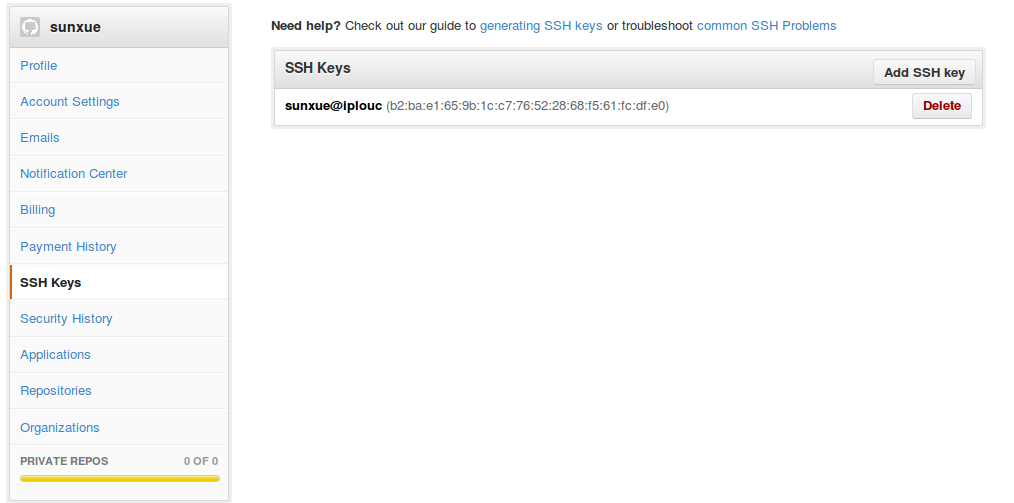
\includegraphics[width=1.0\textwidth]{SSH.png}
\caption{SSH Keys}\label{fig:2}
\end{figure}
\item 把密钥加载到SSH里。在终端输入\lstinline|ssh-add|。
\end{enumerate}

\subsection{通过SSH代理使用GitHub}

\begin{enumerate}
\item ssh配置文件。打开终端,执行:\lstinline|vim ~/.ssh/config|,写入内容:
\begin{plaintext}
Host github.com
ProxyCommand ~/.ssh/ssh-https-tunnel %h %p
Port 443
Hostname ssh.github.com
\end{plaintext}
\item 设置代理地址。执行\lstinline|vim ~/.ssh/ssh-https-tunnel|,内容已在\url{https://github.com/zhenglab/LaTeX\_Git-GitHub-howto}中公布,注意其中的\verb|my $host|和\verb|my $port|改为实验室代理地址和端口)。
\item 测试。在终端输入:\lstinline|ssh -T git@github.com|,此时,若出现权限问题,如图\ref{fig:3},则说明ssh-https-tunnel文件不可执行,此时,可以用命令:\lstinline|chmod +x ~/.ssh/ssh-https-tunnel|来加上执行权限,用命令:\lstinline|ls -al ~/.ssh/ssh-https-tunnel|来查看是否添加成功。
\begin{figure}[!htb] %插图
\centering
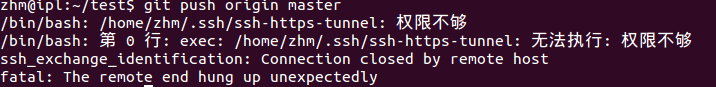
\includegraphics[width=0.8\textwidth]{permission.png}
\caption{权限问题}\label{fig:3}
\end{figure}

若出现如下密匙问题,如图\ref{fig:4},则选择yes,或参考网页\cite{2:misc}来解决。
\begin{figure}[!htb] %插图
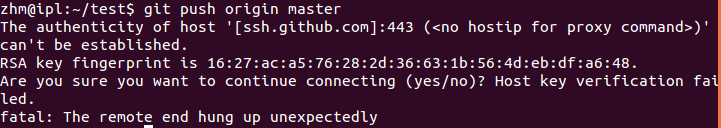
\includegraphics[width=0.8\textwidth]{key.png}
\centering\caption{密匙问题}\label{fig:4}
\end{figure}

若出现图\ref{fig:5},则说明设置成功。
\begin{figure}[!htb] %插图
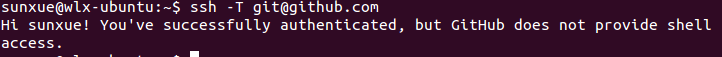
\includegraphics[width=0.8\textwidth]{ssh-success.png}
\centering\caption{设置成功}\label{fig:5}
\end{figure}
\end{enumerate}

\section{Git的安装与配置}

\begin{enumerate}
\item 下载与安装。在Ubuntu 11.10环境下: \lstinline|sudo apt-get install git|。
\item 初次运行Git前的配置。Git提供了一个叫做\lstinline|git config|的工具,用来配置相应的工作环境变量,这些变量可以存放在三个地方\cite{3:misc}:
\begin{itemize}
\item \verb|/etc/gitconfig|文件:系统中对所有用户都普遍适用的配置。若使用\lstinline|git config --system|,读写的就是这个文件。
\item $\sim$\verb|/.gitconfig|文件:用户目录下的配置文件,只适用于该用户。若使用\lstinline|git config --global|,读写的就是这个文件。
\item 当前项目的\verb|git|目录中的配置文件(也就是工作目录中的\verb|.git/config|文件):这里的配置仅仅针对当前项目有效。
\end{itemize}
初次运行Git前一般需要用\lstinline|git config --global|设置用户名和电子邮件地址\cite{1:misc}。
打开终端,输入
\begin{bash}
git config --global user.name "your name here"
git config --global user.email "your email here"
\end{bash}
此时,用\lstinline|git config --list|命令就可以查看是否设置成功。设置成功后,之后每次提交文档或代码时都会引用这两条信息说明是谁提交了更新以及他的电子邮件地址是什么。
\end{enumerate}

\section{Git的使用}
\label{sec:git}

\subsection{初始化仓库}

\begin{enumerate}
\item 在本地创建\verb|Test|目录: \lstinline|mkdir ~/Test|
\item 转到\verb|Test|目录: \lstinline|cd ~/Test|
\item 初始化仓库: \lstinline|git init|
\end{enumerate}

初始化后,在当前目录下会出现一个名为\verb|.git|的隐藏目录,可以通过\lstinline|ls -a|来查看,所有Git需要的数据和资源都存放在这个目录中。不过目前,仅仅是按照既有的结构框架初始化好了里边所有的文件和目录,但我们还没有开始跟踪管理项目中的任何一个文件\cite{4:misc}。

\subsection{跟踪文件与取消跟踪}

对任何一个文件,Git都有三个状态:已提交(committed),已修改(modified),已暂存(staged)。
\begin{description}
\item[已提交] 表示该文件已经被安全地保存在本地数据库中了。
\item[已修改] 表示修改了某个文件,但还没有提交保存。
\item[已暂存] 表示把已修改的文件放在下次提交时要保存的清单中。
\end{description}

可以通过\lstinline|git status|命令来查看文件的状态。

\begin{enumerate}
\item 新建\verb|hello|文档: \lstinline|touch hello|。
\item 写入内容:\lstinline|vim hello|,然后输入\verb|Hello!|保存。
\item 查看文件的状态:\lstinline|git status|,会发现有提示:\verb|Untracked files|,这说明Git没有跟踪\verb|hello|文档。
\item 开始跟踪文件:\lstinline|git add hello|。对于已经跟踪的文件,\lstinline|git add|的意义是把已跟踪的文件放在了暂存区。
\item 查看状态:\lstinline|git status|,会发现有提示:\verb|Changes to be committed|,这说明\verb|hello|文档已经被跟踪了,即放在了暂存区,属于已暂存状态。
\item 若是再修改\verb|hello|文档,比如说将\verb|Hello!|改为\verb|hello world|,此时查看状态时你会发现\verb|hello|有两个状态,一个是未暂存,一个是已暂存。实际上,如果你此时提交,提交的是没有修改的\verb|hello|文档,所以每次对文档做了修改,都应该重新用\lstinline|add|把文档放入暂存区已备提交。
\item 取消跟踪:\lstinline|git rm --cached hello|,此时再查看状态你会发现又回到了原来的状态。
\end{enumerate}

\subsection{提交文件}

使用\lstinline|git commit -m 'message'|命令可以把暂存区的文件提交,此时历史记录里就有此时的文件状态。每次提交实际上就是对项目做了一次快照。message是对这一次的提交给出说明。.git里的\verb|COMMIT-EDITMSG|文件,是最后一次提交时的说明。

可以通过\lstinline|git commit -a -m 'message'|来跳过暂存,直接提交。

\subsection{查看提交历史}

用\lstinline|git log|命令可以查看提交历史。默认不输入参数的话,\lstinline|git log|会按提交时间列出所有的更新,最近的更新排在最上面,同时给出作者的名字和电子邮件地址。

用\lstinline|git log -p|可以查看每次提交的内容差异,用\lstinline|git log -2|则显示最近两次的更新。查看更多关于\lstinline|git log|的参数设置可以通过\lstinline|git help log|。

\subsection{恢复历史版本}
\subsubsection{恢复项目的历史版本}

在进行一个项目时,有时会发现你项目中后几次所做的修改完全是错误的,若想重置到之前某个版本,也就是说删除历史记录中某个版本之后的所有的版本的记录,Git也可以帮你做到。

首先,你可以使用\lstinline|git log|命令查看你想要恢复的版本的哈希值(hash)。Git使用SHA-1算法计算数据的校验和,通过对文件的内容或目录的结构计算出一个SHA-1哈希值,作为指纹字符串。该字串由$40$个十六进制字符($0-9$及a-f)组成,看起来像是:f829d445fa8fdec258e58c61f730bd769e31bdbd。

然后就可以用\lstinline|git reset|命令来恢复到你选中的版本,\lstinline|git reset|命令有很多的参数选项,下面就简单的介绍其中两个,其它选项可以用\lstinline|git help reset|命令查看。

\begin{description}
\item[hard] 选用hard选项来恢复某个版本,会删掉这个版本之后所做的所有的提交,此时项目中的文件也回到了这个版本的状态。查看历史记录(\lstinline|git log|)你会发现,记录中只是记载了这个版本之前的修改。具体做法是,用\lstinline|git log|命令查看想要恢复的版本的哈希值(hash),然后用\lstinline|git reset --hard hash|命令恢复。此时这个版本之后的所有的提交都会被删除。
\item[soft] 选用soft选项来恢复某个版本,删除了历史记录中的这个版本之后的所有版本,但是项目中的最新版本的文件并没有做相应的更改,仍是现在的状态。也就是说,用soft选项后的结果虽然删除了指定版本之后的所有的版本的历史记录,但是,因为项目中保留了最新的版本,所以若是出现了误删,仍可以重新用\lstinline|git add|和\lstinline|git commit|命令重新提交,从而把最新版本加入到提交记录中。
\end{description}

注意,若是在本地恢复了项目了历史版本,也就是说删除了一些历史记录后,若想更新到远程GitHub上,必须使用\lstinline|git push -f origin master|命令(如果远程GitHub中包含你所删除的记录)。f参数是强制执行的意思。因为若不强制执行,就会提示让用\lstinline|git pull|命令把远程项目合并到本地来,这时就会把删掉的记录又重新合并到本地项目的历史记录中,造成记录的混乱。

\subsubsection{恢复单个文件的历史版本}

上面讲到的是恢复整个项目的某个版本,若是想恢复其中某个文件的版本,可以用\lstinline|git log filename|来查看想回到版本的哈希值,然后用\lstinline|git reset --hard hash|来恢复。

\subsection{修改提交说明}

修改最新提交的说明比较简单,只需一条命令即可:\lstinline|git commit --amend|,此时你就可以修改\#号之上的说明,并用Ctrl+X和Y键进行保存。 

若是想修改历史记录中的提交说明,例如,倒数第三次提交说明,则需要几个步骤:
\begin{enumerate}
\item 输入\lstinline|git rebase -i HEAD~2|命令,这句话的意思是衍合到倒数第二次提交,关于衍合的详细解释,可以用\lstinline|git help rebase|查看。此时,你会看到如图\ref{fig:10}的界面。把第一行中的pick改为edit,然后保存,退出(Ctrl+X键和Y键)。注意,此时的这个列表与用\lstinline|git log|查看历史记录时的列表顺序正好相反,所以修改时要注意。
\item 输入\lstinline|git commit --amend|命令,此时就可以修改提交说明,修改后保存。
\item 输入\lstinline|git rebase --continue|命令,完成修改,此时查看历史记录会发现提交说明已经修改成功。

\begin{figure}[!htb] %插图
\centering
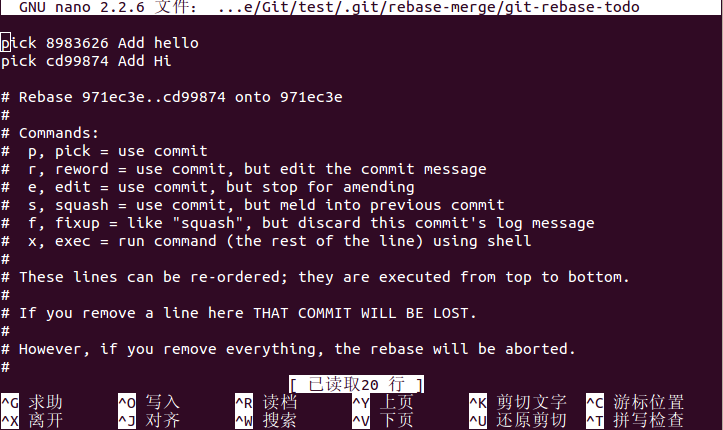
\includegraphics[width=0.9\textwidth]{edit.png}
\caption{}\label{fig:10}
\end{figure}
\end{enumerate}

跟上面提到的恢复历史版本一样,修改以后若想提交到远程GitHub上,而GitHub中包含修改之前的版本时,必须使用\lstinline|git push -f origin master|命令。

\subsection{查看某个历史版本的文件}
Git可以通过打标签的方式查看历史版本的文件,也可以不用打标签。
\begin{description}
\item [打标签]
Git可以对某一时间点上的版本打上标签。若是你觉得当前的版本相对较为成熟,你可以给当前版本打上标签,方便以后查看这个版本。

比如,我们提交了某个项目中的所有文件,然后我们新建标签:
\begin{bash}
git tag -a v1.0 -m 'message'
\end{bash}
此时,我们就可以查看这个版本中的文件内容:
\begin{bash}
git show v1.0:./
\end{bash}
冒号后为项目的路径,./是当前路径的意思,若是想查看这个项目中的某个文件的内容,可以在/后加上文件名。
\item[不打标签]
若想直接查看某个文件的历史版本,Git也可以做到。首先应通过\lstinline|git log|指令找到你想查看的版本的哈希值,比如说: d26673579fa5a8a328a7e36336724548cd7b210f。然后就可以用以下指令来查看了,当然,filename要改成你想查看的文件的文件名。
\begin{bash}
git show :d26673579fa5a8a328a7e36336724548cd7b210f:./filename
\end{bash}
\end{description}
\subsection{忽略文件}

有时编译时产生一些中间文件,如果不想跟踪这些文件,也可以进行设置\cite{5:misc}。在新建一个项目时,养成一个写忽略文件的好习惯,可以有助于减少以后的麻烦,使Git管理更出色。

设置忽略文件有几种不同的方式,这里简单介绍三种。一种是建立\verb|.gitignore|文件,另一种是修改\verb|exclude|文件,还可以设置全局的忽略文件。
\begin{description}
\item[.gitignore] 首先应确保你的忽略文件处于为跟踪状态,若是已跟踪,则用命令\lstinline|git rm --cached filename|来取消跟踪。然后在你的项目仓库下创建\verb|.gitignore|文件:\lstinline|touch .gitignore|。写入你想忽略的文件的扩展名,例如,想忽略所有.log的文件和所有以$\sim$结尾的文件,则写入内容:
\begin{plaintext}
*.log
*~
\end{plaintext}

此时,将不会再跟踪这两类文件。每个项目中的\verb|.gitignore|文件内容可以是不相同的,根据实际情况可以设置想忽略的文件。
\item[exclude] 你也可以在你的项目中的\verb|.git/info/exclude|中设置你的忽略文件,但是这个设置只是当前用户的设置,其他人无法共享。也就是说它无法被提交到GitHub网站上以供别人克隆和使用。
\item[全局忽略文件] 设置全局的\verb|.gitignore|文件可以使你所有的项目都忽略掉你所设置的忽略文件。
\end{description}

参考文献\cite{7:misc}中包含很多种类的\verb|.gitignore|文件的模板,比如\LaTeX等等,可以拷贝下来放在自己的项目中。

我们规定了实验室中使用忽略文件的方式:首先,郑老师在GitHub网站上新建项目的时候会选择忽略文件的类型,这样项目创建成功后,相应的忽略文件就会包含在项目中。我们克隆项目的时候忽略文件就会被克隆到本地。若是需要,可以修改项目中的\verb|.gitignore|文件。

我们可以设置全局的忽略文件来优化我们的设置。打开终端,转到$\sim$目录下,执行\lstinline|git config --global core.excludesfile ~/Linux.gitignore|,然后编辑\verb|Linux.gitignore|文件:\lstinline|vim Linux.gitignore|,写入内容:
\begin{plaintext}
.*
!.gitignore
*~
\end{plaintext}
这样,所有的Git项目中除了\verb|.gitignore|文件之外的其他隐藏文件和以$\sim$结尾的文件在提交到GitHub上时都会被忽略。

\subsection{本地仓库与远程仓库的冲突合并}

有时候我们在用\lstinline|git commit|命令在本地提交之后,想要用\lstinline|git push|提交到远程仓库上时,会发现无法推送的问题\ref{fig:6}。这是因为远程仓库上的版本不是本地版本的上一版本。

\begin{figure}[!htb] %插图
\centering
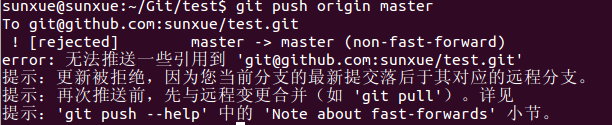
\includegraphics[width=0.9\textwidth]{push-error.png}
\caption{push error}\label{fig:6}
\end{figure}

此时,根据提示,应该用\lstinline|git pull|在终端执行一下,然后会看到提示\ref{fig:7}。

\begin{figure}[!htb] %插图
\centering
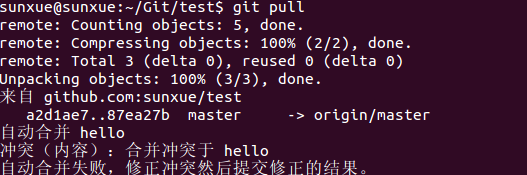
\includegraphics[width=0.9\textwidth]{pull-error.png}
\caption{pull error}\label{fig:7}
\end{figure}

比如说,当前本地仓库有个名为\verb|hello|的文件,里面的内容是hello kitty,hello kitty的前一版本的内容是hello。远程仓库的hello文件的内容是hello world。此时要把本地仓库的\verb|hello|文件提交到远程仓库,即执行\lstinline|git push|和\lstinline|git pull|时就会出现以上错误。此时打开本地仓库中的\verb|hello|文件,可以看到内容如图\ref{fig:8}。

\begin{figure}[!htb] %插图
\centering
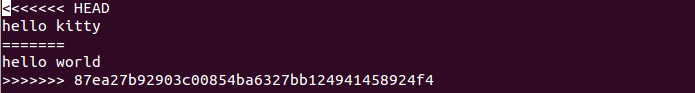
\includegraphics[width=0.9\textwidth]{conflict.png}
\caption{conflict}\label{fig:8}
\end{figure}

其中=====隔开的上半部分是本地仓库中的内容,下半部分是远程仓库上的内容。解决冲突的办法是二者选其一或者整合到一起(====等符号及解释都应该删除)。修改完之后,再进行\lstinline|git add|,\lstinline|git commit|以及\lstinline|git push|就没有问题了。

这种本地仓库与远程仓库的冲突一般是在合并同一个文件的同一部分时,其内容不同造成的。合并同一文件的不同部分或者合并不同文件时,不会产生冲突,此时使用\lstinline|git pull|命令,就可以把GitHub上新更新的内容自动的拉取和合并到本地仓库中。

另外,若用\lstinline|git pull|时出现图\ref{fig:9}情况,可以按Ctrl+X键和Y键保存这个合并信息。

\begin{figure}[!htb] %插图
\centering
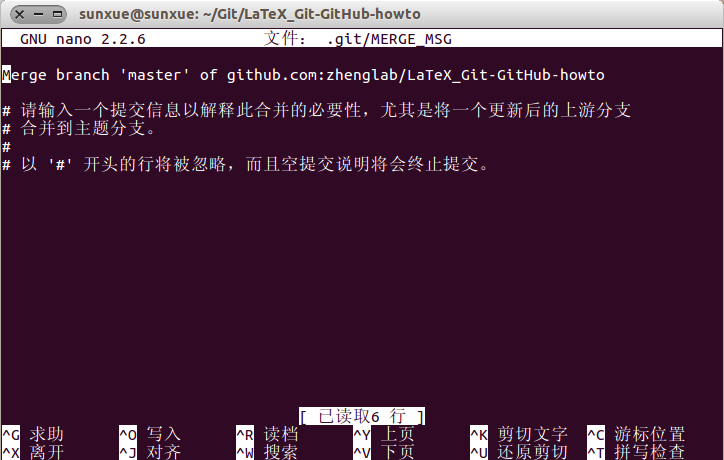
\includegraphics[width=0.9\textwidth]{pull-error1.png}
\caption{pull problem}\label{fig:9}
\end{figure}
\section{实验室中Git和GitHub的使用}

学会上面的用法后,下面就从实验室的使用情况来做简单介绍。

\subsection{克隆已有的仓库}

实验室的GitHub网站为\url{https://github.com/zhenglab/},通常情况下,若是需要你上传一些材料到这个网站,郑老师会新建一个项目仓库供你上传。下面就开始进行操作:
\begin{enumerate}
\item 首先要登陆网站,选择你要克隆的Repositories。
\item 开始克隆。打开终端,转到你想要建立仓库的目录,比如说Git目录,执行\lstinline|git clone git@github.com:zhenglab/ROC_PR.git|,此时在你Git目录下就会生成一个\verb|ROC_PR|的仓库。
\item 从远程拷贝文件\cite{6:misc}。
\begin{itemize}
\item 转到这个仓库:\lstinline|cd ROC_PR|。
\item 告诉Git远程库的名字和地址:
\begin{bash}
git remote add upstream git@github.com:zhenglab/ROC_PR.git
\end{bash}
\item 从远程抓取数据:\lstinline|git fetch upstream|。
\end{itemize}
\item 提交文件。把你想要提交的文档(例如\verb|ROC_PR.pdf|)复制到你的\verb|ROC_PR|文件夹下,执行
\begin{bash}
git add ROC_PR.pdf
git commit -m 'Add ROC_PR.pdf'
git push origin master
\end{bash}
此时,\url{https://github.com/zhenglab/}上的\verb|ROC_PR|仓库中就有了你提交的\verb|ROC_PR.pdf|文档。
\item 要注意的是,每次修改过的文档,都必须执行\lstinline|git add|,\lstinline|git commit|,\lstinline|git push|(推送当前分支到指定远程分支)才能使得GitHub上得到更新。
\end{enumerate}

\subsection{新建仓库}

你也可以在你自己的GitHub上新建一个仓库,然后把本地的文件上传上去。

\begin{itemize}
\item 打开浏览器,转到https://github.com/your name。
\item 点击Respositories选项卡,然后点击New,创建一个新的库。
\item 填写库名(比如Test)和描述,选择Public或者是Private,在Initialize this repository with a README选项前打勾,可以选择添加\verb|.gitignore|文件和\verb|license|,然后点击Create repository,如图\ref{fig:1}。
\begin{figure}[!htb] %插图
\centering
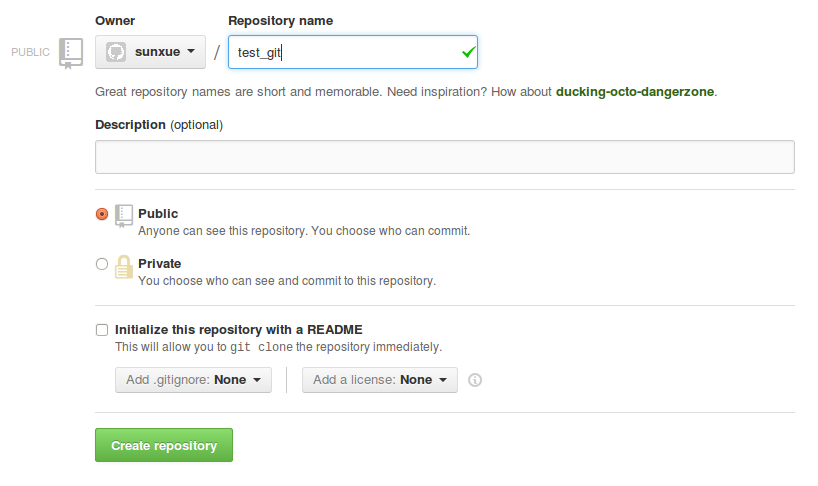
\includegraphics[width=1.0\textwidth]{new.png}
\caption{new repository}\label{fig:1}
\end{figure}
\item 让Git记住远程库的名和地址(前提是你已经在本地仓库中用\lstinline|git commit|提交了你的\verb|hello|文档,参考第\ref{sec:git}章)。
\begin{bash}
git remote add origin git@github.com:Your name/Test.git
\end{bash}
\item 推送到远程库:\lstinline|git push origin master|。
\end{itemize}

以上就是对于Git和GitHub的基本使用,要想了解更多关于Git和GitHub的内容,可以参考\cite{1:misc}\cite{3:misc}。

\bibliographystyle{plain}
\bibliography{Git-GitHub-howto} %加入参考文献

\end{document}

